\section{支持向量机}

\subsection{逻辑回归的缺陷}
\begin{enumerate}
	\item 按照逻辑回归的计算方式,我们得到的是一个分隔线(或平面或超平面\footnote{1维称为线,2维称为平面,更多维就称为超平面}),对于我们的数据点,总有一些点离超平面较近(如点C),有一些点离超平面较远(如点A);对于离超平面较远的点,我们有很大把握保证我们的预测是准确的,但是,对于离超平面较近的点我们就没把握了。
	\begin{figure}[htbp]
		\centering
		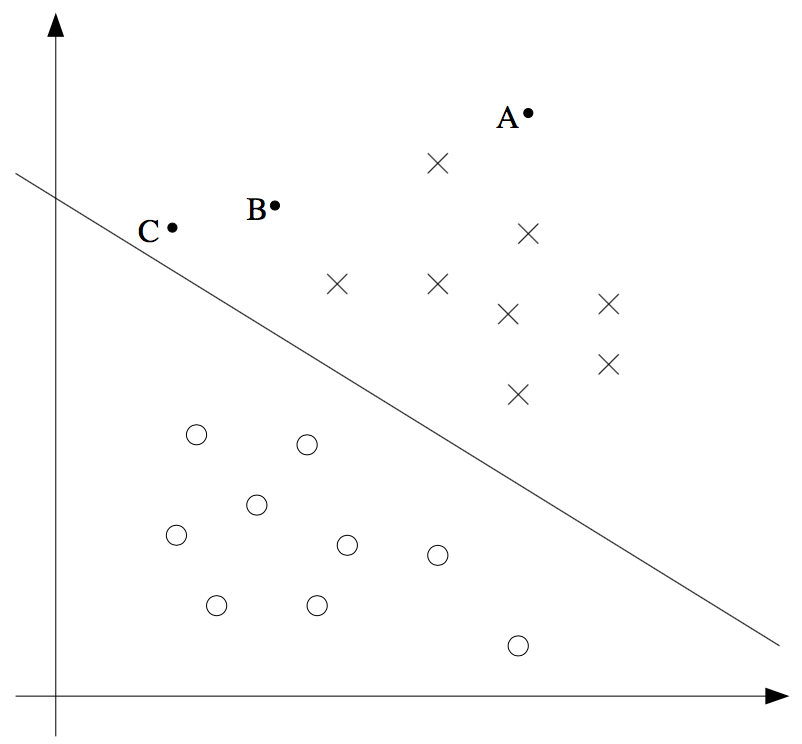
\includegraphics[scale=0.5]{images/逻辑回归缺陷讲述}
		\caption{支持向量机实例用图}
	\end{figure}
\end{enumerate}

\subsection{SVM前言}
\begin{enumerate}
	\item 在后续介绍SVM过程中,为了描述方便,我们对之前逻辑回归的一些描述做了更改
	\item 将$h_\theta(x)$更改为$h_{w,b}(x)$,其中:$w \to \left[\begin{matrix}\theta_1 \\ \theta_2 \\ \vdots \\ \theta_n  \end{matrix}\right]$,$b \to \theta_0$\footnote{此处为了表达方便,使用$\to$来表达类似的对应关系,且勿将其当做等于"$=$"}
	\begin{align}
		h_{w,b}(x) = g(w^Tx+b)
	\end{align}
	\item 将类标签$y$改为$\{-1, 1\}$;将$h=g(w^T+b)$的值从值域$\{0,1\}$切换到$\{-1, 1\}$,其中,$0\to -1$,$1\to 1$
	,且取消原有的$x_0=1$假设。通过此方式将$h(x)$由参数$\theta$变成了参数$(w, b)$,将截距项$b$与其他项分隔开,以便分析
\end{enumerate}

\subsection{Margin介绍}
\subsubsection{函数间隔}
\begin{enumerate}
	\item 对于数据点$(x^{(i)}, y^{(i)})$,其函数间隔定义为:
	\begin{align}
		\hat{\gamma}^{(i)} = y^{(i)}(w^Tx^{(i)} + b)
	\end{align}
	\item 对于$y^{(i)}=1$的点,为了让函数间隔$\hat{\gamma}$越大,我们需要让$w^Tx^{(i)} + b$正向越大;
	\item 对于$y^{(i)}=-1$的点,为了让函数间隔$\hat{\gamma}$越大,我们需要让$w^Tx^{(i)} + b$负向越大;
	\item 对于给定的训练集$S=\{(x^{(i)}, y^{(i)}); \quad i = 1, \dots, m\}$,我们将其中最小的函数间隔记为$\hat{\gamma}$:
	\begin{align}
		\hat{\gamma} = \min_{i=1,\dots,m}\hat{\gamma}^{(i)}
	\end{align}
	\item 对于函数间隔,若将参数$(w,b)$扩大2倍2为$(2w,2b)$,函数间隔的值$\hat{h}_{w,b}(x)$也变成了原来的2倍,但实际上,这对训练的效果并没有影响,原来错误的现在还是错误
\end{enumerate}

\subsubsection{几何间隔}
\begin{enumerate}
	\item 几何间隔表示为$\gamma^{(i)}$\footnote{与函数间隔相比,少了头顶的帽子: $\hat{ }$}。
	\item 对于数据点$(x^{(i)}, y^{(i)})$,其几何间隔定义为\footnote{证明过程略}:
	\begin{align}
		\gamma^{(i)} &= \frac{\hat{\gamma}^{(i)}}{\|w\|}  \\
		&= \frac{y^{(i)}(w^Tx^{(i)} + b)}{\|w\|}  \\
		&=  y^{(i)} \left(\left(\frac{w}{\|w\|}\right)^T x^{(i)} + \frac{b}{\|w\|}\right)
	\end{align}
	\item 当$\|w\|=1$时,几何间隔与函数间隔相等
	\item 相较于函数间隔,几何间隔任意缩放参数$(w,b)$不影响$h_{w,b}(x)$的值;鉴于此性质,我们可以在训练时对$w, b$视需求进行缩放
	\item 同样,对于给定的训练集$S=\{(x^{(i)}, y^{(i)}); \quad i = 1, \dots, m\}$,我们将其中最小的几何间隔记为$\gamma$:
	\begin{align}
		\gamma = \min_{i=1,\dots,m}\gamma^{(i)}
	\end{align}
\end{enumerate}

\subsubsection{函数间隔\&几何间隔}
\begin{enumerate}
	\item 当预测正确时,二者都是正值;当预测错误是,二者都是负值。
\end{enumerate}

\subsubsection{对SVM设计函数间隔、几何间隔原因的思考}
{\color{red}{注意,此部分内容仅仅是我自己的理解,不见得正确,请批判性地看。}}
\begin{enumerate}
	\item 与之前的逻辑回归类似,此处$w^Tx+b=0$是用来判断预测值$h_{w,b}(x)$取1或-1的分界线:若$w^Tx+b\geq0$,则通过激活函数$g(z)$让$h_{w,b}(x)=g(w^Tx+b)=1$,反之,让$h_{w,b}(x)=-1$。$w^Tx+b=0$相当于门槛的角色,没过门槛是一个世界,过了门槛又是另一个世界
	% \item 与前面逻辑回归一样,$w^Tx+b$与$\theta^Tx$计算出来的结果意义一样,且都是通过激活函数$g(z)$(虽然两者的$g(z)$形式不一样)来得到预测值;
	\item 但是,两者的激活函数$g(z)$不一样,其得到的结果也不一样,逻辑回归的$g(z)$得到的是概率值,后续也是通过让概率值达到最大来优化算法;
	\item SVM的$g(z)$得到的结果是一个我也不知道代表什么意义的值,后续优化的对象是预测值与门槛$w^Tx+b=0$的几何间隔
	\item 但是SVM优化的几何间隔又与线性回归中使用点与点间的距离$h_\theta(x^{(i)})-y^{(i)}$不大一样:它除了与线性回归类似计算了与{\color{red}{门槛}}的距离$w^Tx^{(i)}-b-0$\footnote{此处计算的是与{\color{red}{门槛}}的距离,对于门槛,$w^Tx-b$的值为0}之外,还乘以了它的实际值$y^{(i)}$,$y^{(i)}$的出现可以纠正它的正负号,若预测正确(即预测值与实际值在门槛的同一边),则得到的结果为正值;否则为负值,将此定义为函数间隔;又因为让函数间隔最大化不一定能够得到最优的门槛(总有些投机倒把的通过增大$w,b$来达到目的),于是我们又对函数间隔除以$\|w\|$,解决了这个Bug,将此定义为几何间隔。于是对SVM的优化就是对几何间隔最大值的优化\footnote{为什么对线性回归的优化是取最小值,而对SVM的优化是取最大值?这就是我们要能理解每一步推理目的的原因了}。
\end{enumerate}




















